%%%%%%%%%%%%%%%%%%%%%%%%%%%%%%%%%%%%%%%%%%%%%%%%%%%%%%%%%%%%%
% Demostración de la NP-Completitud
% del problema del Circuito Hamiltoniano
% (Presentation)
% Complejidad Computacional
% Universidad de La Laguna
%
% -- Autores
% Carlos Domínguez García (alu0100966589@ull.edu.es)
% Daute Rodríguez Rodríguez (alu0100973914@ull.edu.es)
% Alberto Jesús González Álvarez (alu0100949568@ull.edu.es)
% Cristian Manuel Abrante Dorta (alu0100945850@ull.edu.es)
%%%%%%%%%%%%%%%%%%%%%%%%%%%%%%%%%%%%%%%%%%%%%%%%%%%%%%%%%%%%%

\documentclass{beamer}
\mode<presentation> {
\usetheme{Madrid}
}

% imported packages
\usepackage{pgfplots}
\pgfplotsset{compat=1.11}
\usepackage{mathrsfs}
\usetikzlibrary{arrows}
\usepackage{graphicx}
\usepackage[utf8]{inputenc}


\title[HC $\mathcal{NP}$-Completitud]{Demostración de la $\mathcal{NP}$-Completitud del problema del Circuito Hamiltoniano}
\subtitle{Complejidad Computacional}
\author[C.D.G., D.R.R., A.G.A., C.A.D.]{
    Carlos Domínguez García,\\
    Daute Rodríguez Rodríguez,\\
    Alberto Jesús González Álvarez,\\
    Cristian Manuel Abrante Dorta
}

\institute[ULL]{Universidad de La Laguna}
\date{9 de enero de 2019}

\begin{document}

\begin{frame}
    \titlepage
\end{frame}

\begin{frame}{Índice}
    \tableofcontents
\end{frame}

\section{Introduction}
\subsection{Motivación}
\begin{frame}{Motivación}
    El problema HC consite en determinar si en un grafo dado (dirigido o no dirigido) existe un \textbf{Circuito Hamiltoniano}. \\
    \vfill
    El estudio de este problema tiene diversas aplicaciones, en parte debido a su estrecha relación con el TSP (Traveling Salesman Probem):
    \begin{block}{Aplicaciones}
        \begin{itemize}
            \item Problemas de rutas.
            \item Problemas de logística.
            \item Problemas de asignación de trabajos.
            \item Problemas de secuenciación de ADN.
        \end{itemize}
    \end{block}
\end{frame}

\subsection{Descripción informal}
\begin{frame}{Descripción informal}
    \begin{definition}
        Un \textbf{circuito hamiltoniano} es un camino a través de los vértices de un grafo, de tal forma que cada vértice \textbf{se visite una sola vez}, y este comience y termine en el mismo vértice.
    \end{definition}
    Se nombró en honor al matemático William Rowan Hamilton (1805 - 1865), quien fromuló el problema de encontrar una \textbf{secuencia de vértices de un icosaedro}, de tal forma que solo se visitaran una vez.
    \begin{columns}
        \column{0.5 \linewidth}
        \begin{figure}
            \centering
            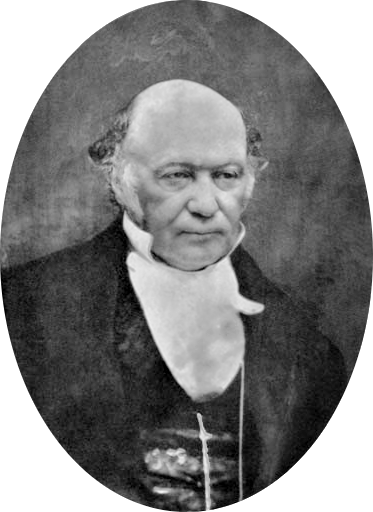
\includegraphics[scale=0.18]{images/william-rowan-hamilton.png}
        \end{figure}
        \column{0.5 \linewidth}
        \begin{figure}
            \centering
            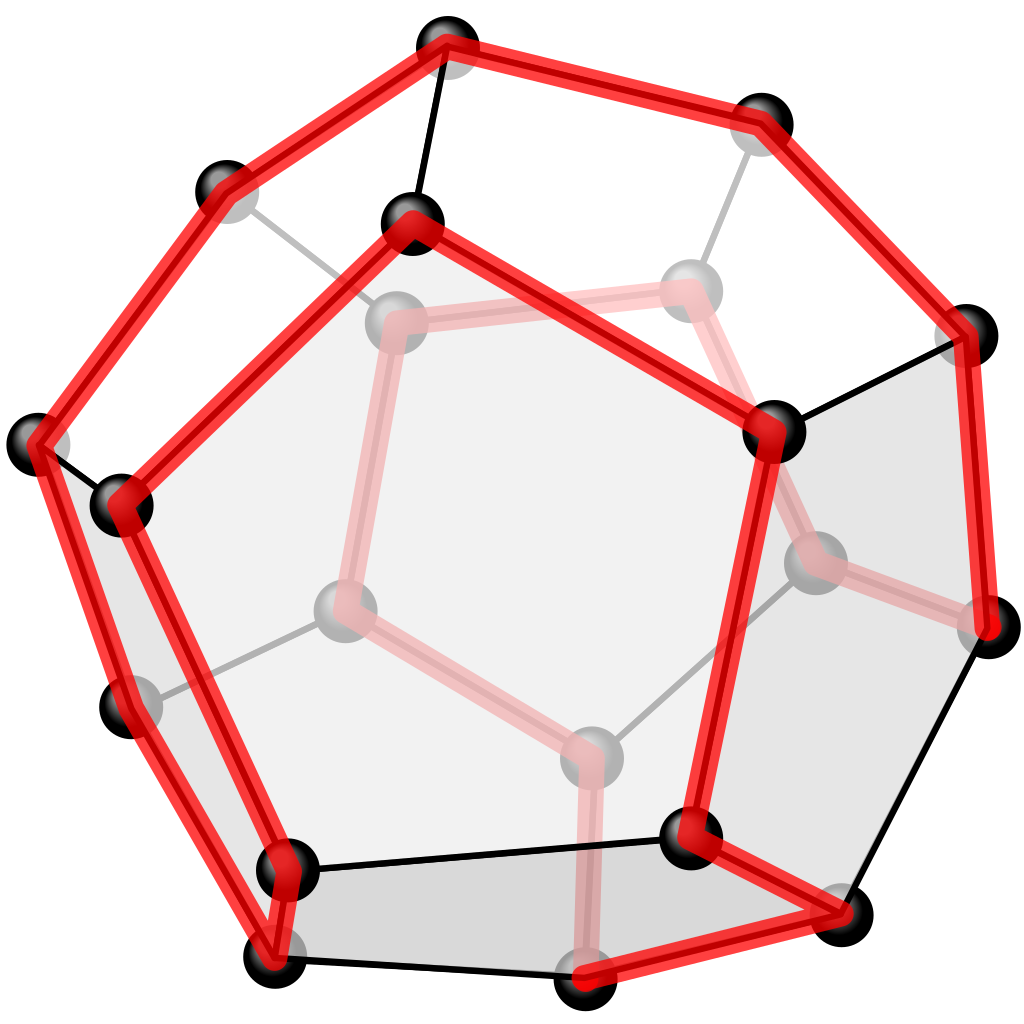
\includegraphics[scale=0.08]{images/icosaedro.png}
        \end{figure}
    \end{columns}
\end{frame}

\subsection{Descripcion formal}
\begin{frame}{Descripción formal}
    La formulación del problema es la siguiente:
    \begin{block}{Instancia}
        La entrada es un grafo:
        \[G=(V, E)\]
        \[V = \{v_1, v_2, \dots, v_n\} \quad |V| = n\]
        \[E = \{\{u, v\} : u, v \in V\}\]
    \end{block}
    \begin{block}{Pregunta}
        \begin{center}
            \textit{¿Contiene G un Camino Hamiltoniano?}\\
            Es decir, contiene G una secuencia ordenada $\displaystyle <v_1, v_2, \dots, v_n>$,
            de tamaño $|V| = n$, tal que:
            \[\{v_n, v_1\} \in E \land \{v_i, v_{i+1}\} \in E \quad \forall i, 1 \le i < n\]
        \end{center}
    \end{block}
\end{frame}

\section{Demostración de $\mathcal{NP}$-Completitud}
\subsection{Introducción}

\begin{frame}{Introducción}
    \begin{figure}
        \centering
        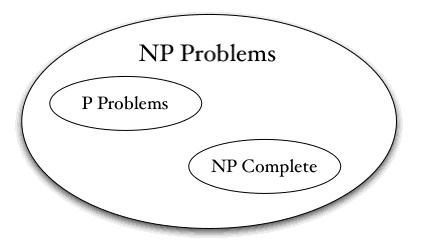
\includegraphics[scale=0.7]{images/p-np.jpg}
        \caption{Diagrama $\mathcal{P} - \mathcal{NP}$}
    \end{figure}
\end{frame}

\begin{frame}{Introducción}
    Para demostrar que un problema ($p$) es $\mathcal{NP}\textbf{-Completo}$, se tiene que satisfacer estas condiciones:
    \vfill
    \begin{enumerate}[I]
        \item El problema pertenece a $\mathcal{NP}$, es decir que existe una \textbf{máquina de Turing no detrminista} que resuelve el problema en tiempo polinomial.
        \[p \in \mathcal{NP}\]
        \item Existe una \textbf{reducción polinomial} de cada uno de los problemas de $\mathcal{NP}$
        a $p$:
        \[\forall p' \in \mathcal{NP}, \quad p' \propto p\]
    \end{enumerate}
\end{frame}

\begin{frame}{Introducción}
    Para realizar la demostración, transformaremos el problema del \textbf{Vertex Cover} en el problema del \textbf{Circuito Hamiltoniano}.
    \only<1> {
        \begin{figure}
            \centering
            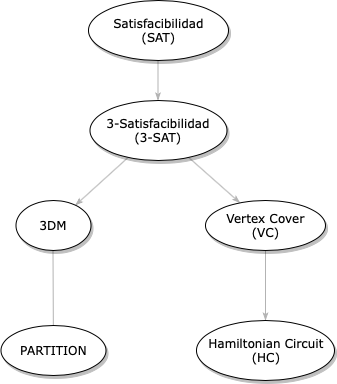
\includegraphics[scale=0.4]{images/NP-Completo-1.png}
            \caption{Diagrama de problemas $NP$-Completo}
            \label{fig:my_label}
        \end{figure}
    }

    \only<2> {
        \begin{figure}
            \centering
            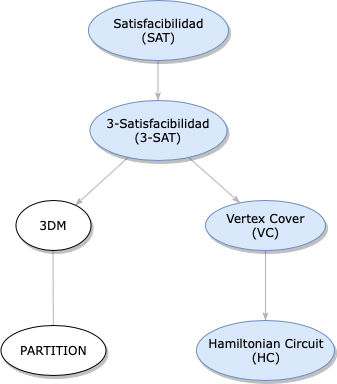
\includegraphics[scale=0.4]{images/NP-Completo-2.png}
            \caption{Diagrama de problemas $NP$-Completo}
            \label{fig:my_label}
        \end{figure}
    }
\end{frame}

\subsection{Vertex Cover}
\begin{frame}{Vetex Cover}
    Definiremos brevemente en que consiste el problema del Vertex Cover (VC):
    \begin{block}{Entrada}
        La entrada es un grafo $G = (V, E)$ y un entero $K \in \mathbb{N},  \quad K \le |V|$
    \end{block}
    \begin{block}{Pregunta}
        \begin{center}
            \textit{¿Existe un vertex Cover de tamaño $K$?}
        \end{center}
        Es decir, ¿podemos encontrar un subconjunto $V'$ de vértices, de tal forma que cada arista es incidente en al menos uno de los vértices del conjunto?
        \[ \exists V' \subseteq V, \quad |V'| \le K : \{u,v\} \in E \to (u \in V') \lor (v \in V')\]
    \end{block}
    Este problema está probado que pertenece a $\mathcal{NP}$-Completo:
    \[VC \in \mathcal{NP}-Completo\]
\end{frame}

\subsection{Demostración de I}
\begin{frame}{Demostración de I}
    \begin{block}{Condición I de $\mathcal{NP}$-Completitud}
        \[HC \in \mathcal{NP}\]
    \end{block}
    Para probar esto, basta con encontrar un \textbf{algoritmo de fuerza bruta}, que compruebe todas las permutaciones de vértices, lo cual presenta una complejidad temporal de:
    \[\mathcal{O}(n!)\]
    Dada un conjunto de vértices concreto, se puede comprobar si es un Camino Hamiltoniano \textbf{en tiempo polinomial}.
\end{frame}

\subsection{Demostración de II}
\begin{frame}{Demostración de II}
    \begin{block}{Condición II de $\mathcal{NP}$-Completitud}
        \[\forall p' \in \mathcal{NP}, \quad p' \propto p\]
        Lo que es equivalente a:
        \[VC \propto HC\]
        Porque $VC \in \mathcal{NP}-Completo$
    \end{block}
    Partiendo del grafo de entrada ($G = (V, E)$) y el entero $K$, nuestra demostración consistirá en \textbf{construir en tiempo polinomial} un grafo $G' = (V', E')$, de tal forma que, $G'$ tendrá un circuito hamiltoniano sí y solo sí, $G$ tiene un Vertex Cover de tamaño $K$ o inferior.
    \vfill
    Esta demostración se basará en la \textbf{construcción de componentes}.
\end{frame}

\subsubsection{selectores}
\begin{frame}{Demostración de II (Selectores)}
    El primer conjunto de componentes será el de los \textbf{selectores}, el cual será un conjunto de vértices.
    \[\{a_1, a_2, \cdots ,a_K\}\]
    Utilizado para seleccionar los $K$ vértices del conjunto $V$ de $G$.
    \[\{a_i : 1 \le i \le K \}\]
\end{frame}

\subsubsection{cover-testing}
\begin{frame}{Demostración de II (Componente cover-testing)}
    Construimos un compoenente \textbf{cover testing} por cada arista en $E$ ($\forall e \in E$).
    Utilizados para garantizar que al menos uno de los vértices de esa arista está entre
    los $K$ vértices seleccionados.\\
    \vfill
    \begin{block}{Componente Cover-Testing}
        Está formado por:
        \begin{itemize}
            \item Un conjunto ($V'_e$) de doce vértices.
            \item Un conjunto ($E'_e$) de catorce aristas.
        \end{itemize}
    \end{block}
\end{frame}

\begin{frame}{Demostración de II (Componente cover-testing)}
    \begin{block}{}
        \[\forall e = \{u, v\} \in E\]
    \end{block}
    Construimos un \textbf{cover-testing} de doce vértices definidos como:
    \[V'_e = \{(u, e, i),(v,e,i) : i \le i \le 6\}\]
    \begin{figure}
        \centering
        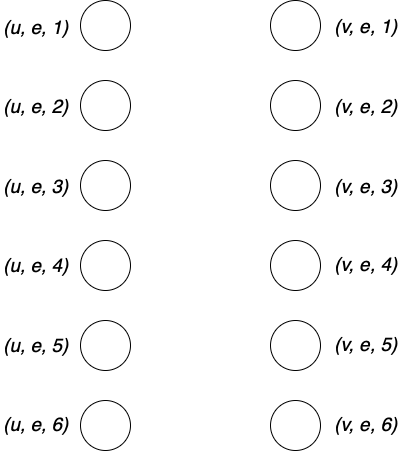
\includegraphics[scale=0.3]{images/cover-testing-1.png}
        \label{fig:my_label}
    \end{figure}
\end{frame}

\begin{frame}{Demostración de II (Componente cover-testing)}
    \begin{block}{}
        \[\forall e = \{u, v\} \in E\]
    \end{block}
    Construimos un \textbf{cover-testing} de catorce aristas definidas como:
    \begin{center}
        \begin{math}
            E'_e = \{\{(u,e,i), (u,e, i+1)\},\{(v,e,i),(v,e,i+1)\} : i \le i < 6\} \\
            \cup \quad \{\{(u,e,3), (v,e,1)\},\{(v,e,3),(u,e,1)\}\} \\
            \cup \quad \{\{(u,e,6), (v,e,4)\},\{(v,e,6),(u,e,4)\}\}
        \end{math}
    \end{center}
    \begin{figure}
        \centering
        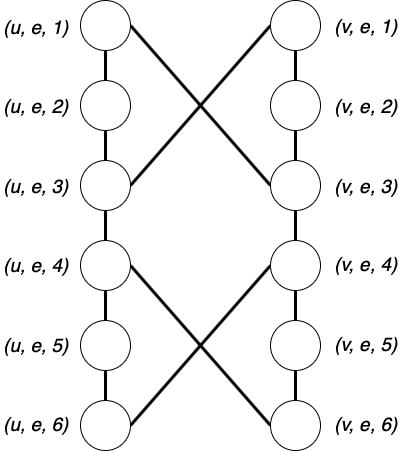
\includegraphics[scale=0.25]{images/cover-testing-2.png}
        \label{fig:my_label}
    \end{figure}
\end{frame}

\begin{frame}{Demostración de II (Componente cover-testing)}
    Los únicos vértices que aparecerán en alguna otra arista de $G'$ serán:
    \[(u,e,1) \quad (v,e,1) \quad (u,e,6) \quad (v,e,6)\]
    De esta forma, se garantiza que cualquier \textbf{circuito hamiltoniano} de $G'$,
    recorrerá los vértices de $E'_e$, solo en una de estas tres formas:
    \begin{columns}
        \column{0.33 \linewidth}
        \begin{figure}
            \centering
            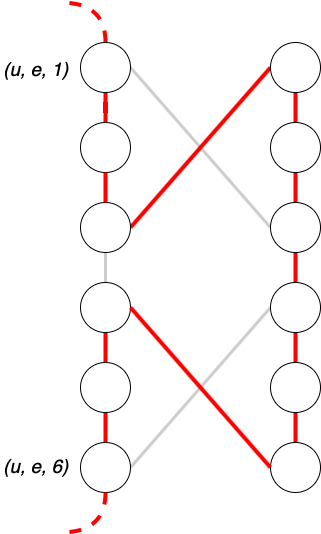
\includegraphics[scale=0.2]{images/cover-testing-3.png}
            \caption{$u$ está en el cubrimiento}
            \label{fig:my_label}
        \end{figure}
        \column{0.33 \linewidth}

        \begin{figure}
            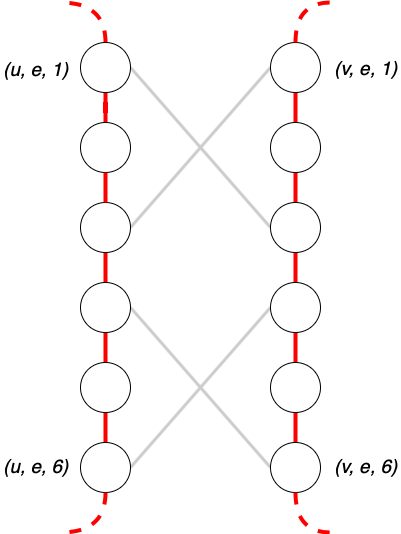
\includegraphics[scale=0.2]{images/cover-testing-4.png}
            \caption{$u$ y $v$ están en el cubrimiento}
            \label{fig:my_label}
        \end{figure}
        \column{0.33 \linewidth}
        \begin{figure}
            \centering
            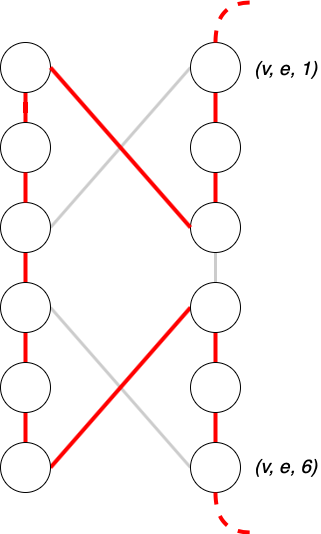
\includegraphics[scale=0.2]{images/cover-testing-5.png}
            \caption{$v$ está en el cubrimiento}
            \label{fig:my_label}
        \end{figure}
    \end{columns}
\end{frame}

\subsubsection{Conexiones}
\begin{frame}{Demostración de II (Conexiones)}
    En primer lugar, se ordenan las aristas incidentes en cada vértice de manera arbitraria:
    \[\forall v \in V, \quad <e_{v[1]}, e_{v[2]}, \cdots, e_{v[deg(v)]}>\]
    Luego se construye el conjunto $E'_v$ de aristas que conectan \textbf{componentes cover-testing}:
    \[E'_v = \{\{(v, e_{v[i]}, 6), (v, e_{v[i+1]},1)\} : 1 \le i < deg(v)\}\]
    Finalmente, se conectan los finales de estos caminos con cada uno de \textbf{los selectores}:
    \[E'' = \{\{a_i, (v,e_{v[1], 1})\},\{a_i, (v,e_{v[deg(v)]}, 6)\} : 1 \le i \le K, v \in V \}\]
\end{frame}

\subsubsection{Prueba}
\begin{frame}{Demostración de II}
    Una vez hemos definido los componentes y concexiones, defnimos $G'$ como:
    \begin{block}{$G'$}
        \[G' = (V', E')\]
        \[V' = \{a_i : 1 \le i \le K\} \cup (\bigcup_{e \in E} V'_e)\]
        \[E' = (\bigcup_{e \in E} E'_e) \cup (\bigcup_{v \in V} E'_v) \cup E''\]
    \end{block}
\end{frame}

\begin{frame}{Demostración de II}
    \begin{block}{Demostración}
        La demostración de II consiste en que si existe un VC de tamaño $K$ en $G$,
        entonces ha de existir un HC en $G'$.
    \end{block}
    Sea $V^* \subseteq V$ un Vertex Cover en $G$, de tamaño $K$: $V^* = \{v_1,v_2, \cdots, v_k \}$\\
    \begin{block}{}
        Para cada \textbf{cover-testing}, se eligen los nodos dependiendo de la pertenencia al conjunto $V'$.\\
        Luego se eligen las siguientes aristas:
        \begin{itemize}
            \item $\{a_i, (v_i, e_{v_i[1]}, 1)\}, \quad 1 \le j \le K$
            \item $\{a_{i+1}, (v_1, e_{v_i[deg(v_i)]}, 6)\} \quad 1 \le i < K$
            \item $\{a_1, (v_K, e_{v_K[deg(v_K)]}, 6)\}$
        \end{itemize}
    \end{block}
    \begin{block}{}
        \begin{center}
            Estas componentes formarían un \textbf{Circuito Hamiltoniano}.
        \end{center}
    \end{block}
\end{frame}

\subsection{Ejemplo}
\begin{frame}{Ejemplo}
    En el ejemplo utilizaremos el grafo siguiente:
    \[G = (V, E) \quad V = \{v_1, v_2, v_3, v_4\} \quad E = \{e_1, e_2, e_3, e_4\}\]
    \begin{figure}
        \centering
        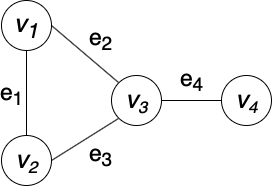
\includegraphics[scale=0.6]{images/example-1.png}
        \label{fig:my_label}
    \end{figure}
\end{frame}

\begin{frame}{Ejemplo}
    El cual tiene un vertex cover ($V^* \subseteq V$):
    \[G = (V, E) \quad V^* = \{v_1, v_2\}\]
    \begin{figure}
        \centering
        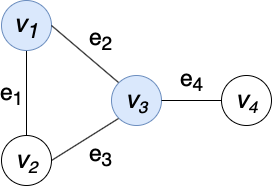
\includegraphics[scale=0.6]{images/example-2.png}
        \label{fig:my_label}
    \end{figure}
\end{frame}

\begin{frame}{Ejemplo}
    Construimos el grafo $G' = (V', E')$:
    \begin{block}{}
        Construimos las componentes \textbf{cover-testing} ($\forall e \in E$)
    \end{block}
    \begin{figure}
        \centering
        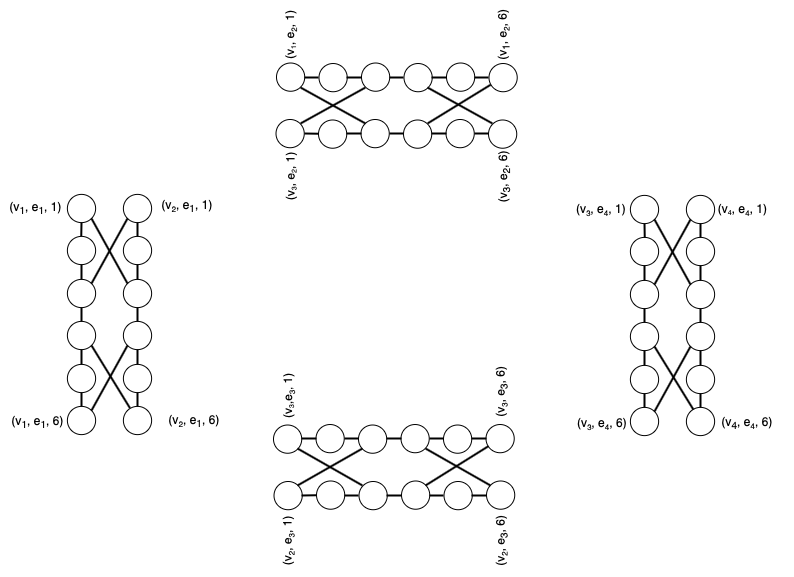
\includegraphics[scale=0.3]{images/example-3.png}
    \end{figure}
\end{frame}

\begin{frame}{Ejemplo}
    Construimos el grafo $G' = (V', E')$:
    \begin{block}{}
        Conectamos los componentes cover-testing: $E'_v = \{\{(v, e_{v[i]}, 6), (v, e_{v[i+1]},1)\} : 1 \le i < deg(v)\}$
    \end{block}
    \begin{figure}
        \centering
        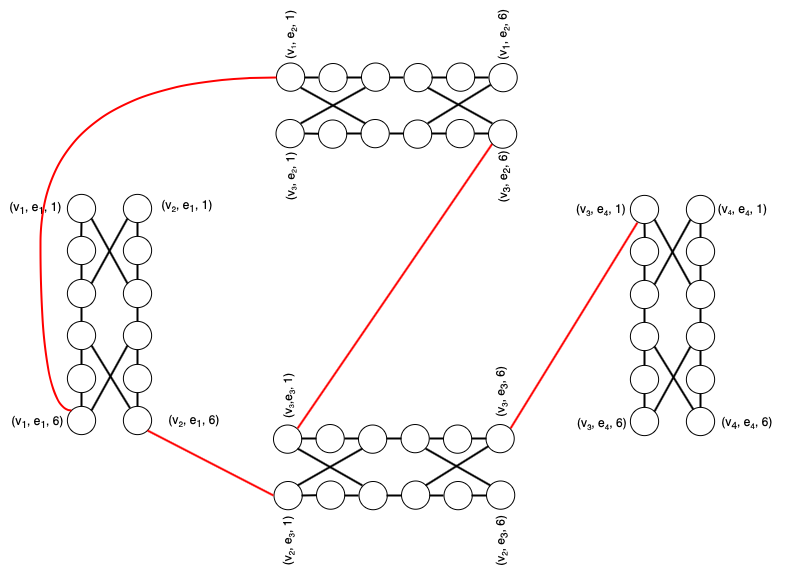
\includegraphics[scale=0.23]{images/example-4.png}
    \end{figure}
\end{frame}

\begin{frame}{Ejemplo}
    Construimos el grafo $G' = (V', E')$:
    \begin{block}{}
        Conectamos los componentes cover-testing con los selectores:
        $E'' = \{\{a_i, (v,e_{v[1], 1})\},\{a_i, (v,e_{v[deg(v)]}, 6)\} : 1 \le i \le K, v \in V \}$
    \end{block}
    \begin{figure}
        \centering
        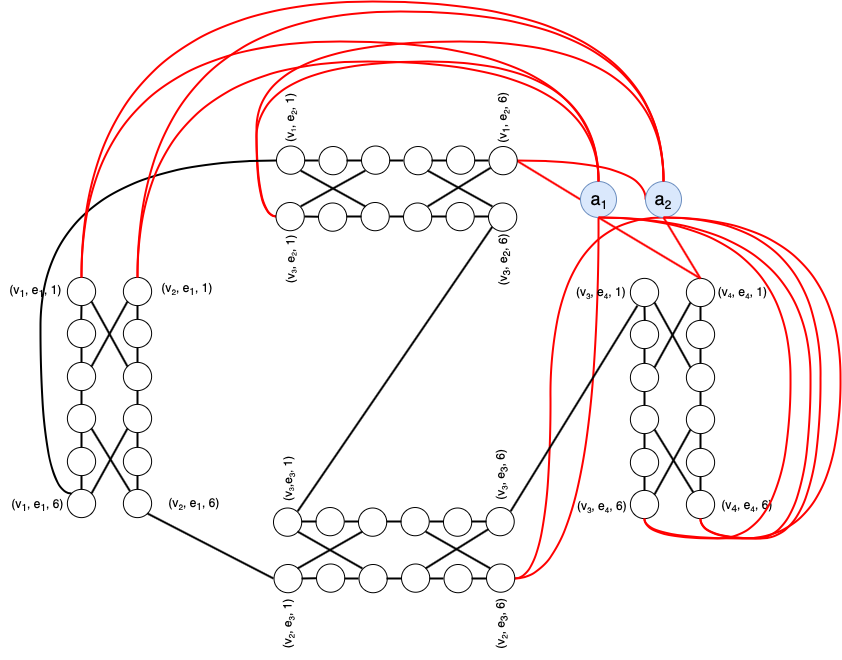
\includegraphics[scale=0.23]{images/example-5.png}
    \end{figure}
\end{frame}

\begin{frame}{Ejemplo}
    Determinamos el circuito hamiltoniano a partir de $V^*=\{v_1, v_3\}$:
    \begin{block}{}
        Elegimos los nodos de los cover-testing que pertenecen a $V^*$
    \end{block}
    \begin{figure}
        \centering
        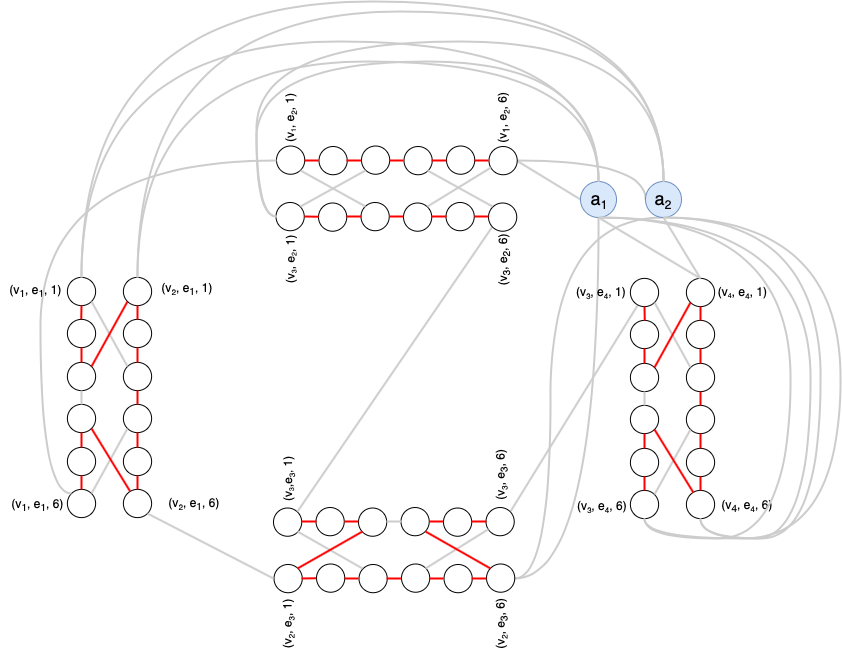
\includegraphics[scale=0.23]{images/example-6.png}
    \end{figure}
\end{frame}

\begin{frame}{Ejemplo}
    Determinamos el circuito hamiltoniano a partir de $V^*=\{v_1, v_3\}$:
    \begin{block}{}
        Elegimos \textbf{las conexiones} entre cover-testing y con los selectores.
    \end{block}
    \begin{figure}
        \centering
        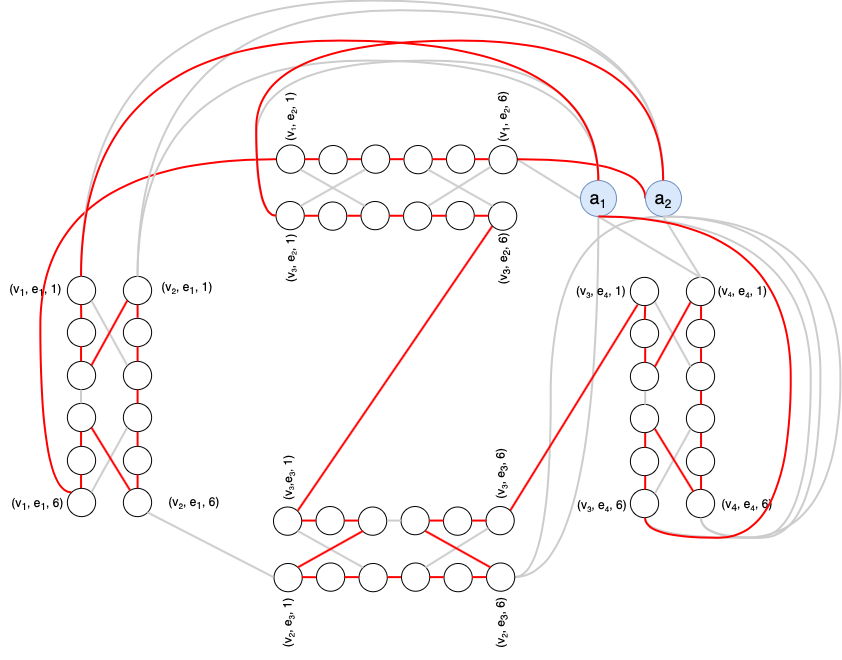
\includegraphics[scale=0.23]{images/example-7.png}
    \end{figure}
\end{frame}

\begin{frame}[allowframebreaks]
    \frametitle<presentation>{Referencias}
    \begin{thebibliography}{10}
        \beamertemplatebookbibitems
        \bibitem{GareyJohnson}
             Michael Garey, David S. Johnson.
            \newblock {\em Computers and Intractability: A Guide to the Theory of NP-Completeness}.
            \newblock W. H. Freeman and Company, 1979.
        \beamertemplatearticlebibitems
        \bibitem{Jemand2000}
            Richard M. Karp.
            \newblock Reducibility Among Combinatorial Problems.
            \newblock {\em Complexity of Computer Computations}, pp:85-103, 1972.
  \end{thebibliography}
\end{frame}

\begin{frame}{}
    \centering \Huge
    \emph{¿Preguntas?}
    \vfill
    \usebeamerfont{institute} Carlos Domínguez García: \url{alu0100966589@ull.edu.es}\\
    \usebeamerfont{institute} Daute Rodríguez Rodríguez: \url{alu0100973914@ull.edu.es}\\
    \usebeamerfont{institute} Alberto Jesús González Álvarez: \url{alu0100949568@ull.edu.es }\\
    \usebeamerfont{institute} Cristian Manuel Abrante Dorta: \url{alu0100945850@ull.edu.es}\\
\end{frame}

\end{document}
